%!TEX root = ../tesis.tex
\section{Otros Modelos de Procesos}
\label{sec:otrosModelos}

Otros enfoques han sido desarrollados para el problema de reconocimiento del habla. En las secciones que siguen
se presentan algunos de estos modelos.

\subsection{Distorsi\'on Din\'amica Temporal}
\label{sec:dtw}

La \gls{dtw} es una t\'ecnica t\'ipica del enfoque basado en comparaci\'on de 
patrones \cite{GaikwadAReview2010}. 
Este m\'etodo permite encontrar una alineaci\'on \'optima entre dos secuencias que pueden variar en 
tiempo y velocidad, bajo ciertas restricciones \cite{MullerInformation2007}.
Las secuencias se distorsionan de manera no lineal con respecto a la dimensi\'on tiempo para determinar 
una medida de similitud independiente a ciertas variaciones no lineales que ocurran sobre la 
dimensi\'on tiempo \cite{AnusuyaSpeech2009}.

Este algoritmo forma un espacio de bidimensional $C$, denominado matriz de costo, para dos secuencias 
$X$ e $Y$ que varian en el tiempo. El objetivo es encontrar
una alineaci\'on entre $X$ e $Y$ de costo total (suma de distancias locales entre elementos) m\'inimo. 
Formalmente a esta alineaci\'on se la conoce como trayectoria de
deformaci\'on, consiste en una secuencia que satisface tres condiciones: restricci\'on de punto final, 
monoton\'ia y tama\~no de paso \cite{MullerInformation2007}. 
En la figura~\ref{figure:dtw} se puede observar una representaci\'on gr\'afica del problema.

\begin{figure}[H]
\centering
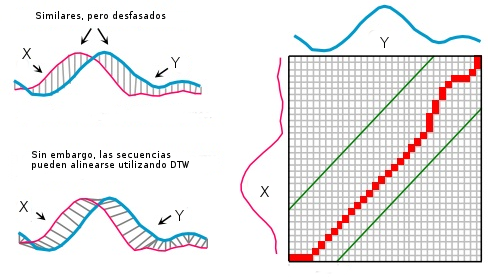
\includegraphics[width=0.8\linewidth]{./graphics/dtw.png}
\caption[Alineaci\'on de secuencias mediante distorsi\'on din\'amica temporal.]{A la izquierda 
    se pueden observar dos secuencias similiares pero desfasadas. Para alinear estas secuencias 
    se construye la matriz $C$ y se busca la trayectoria de deformaci\'on. 
    Gr\'afico modificado de \cite{ThanawinDTW}.}
\label{figure:dtw}
\end{figure}

Para el reconocimiento del habla basado en \gls{dtw} se utilizan tambi\'en los vectores de 
caracter{\'\i}sticas espectrales, los cuales pueden obtenerse de manera similar al proceso 
basado en \gls{hmm} \cite{Hachkar2011}.

Posteriormente, se calcula la distancia entre los vectores de caracter{\'\i}sticas 
espectrales correspondientes a la entrada ac\'ustica y los vectores de caracter{\'\i}sticas 
espectrales correspondientes a las grabaciones de entrenamiento, a los que se denomina plantillas. 
Este paso se realiza mediante el algoritmo \gls{dtw} \cite{Muda2010}.

La secuencia de plantillas para la cual se obtiene la menor distancia a la entrada ac\'ustica,
permite determinar la secuencia de palabras pronunciadas.

La definici\'on de un conjunto de plantillas para el lenguaje que se desea reconocer es uno de
los principales problemas del reconocimiento del habla basado en \gls{dtw}, en particular cuando 
se cuenta con varias grabaciones de una misma palabra \cite{Abdulla2003}. 
Algunas posibles soluciones a este problema son \cite{Abdulla2003}:

\begin{itemize}
    \item Utilizar m\'as de una plantilla por palabra, lo cual resulta ineficiente con el aumento del
    n\'umero de grabaciones.
    \item Combinar las plantillas utilizando cuantizaci\'on vectorial, lo cual requiere de un gran
    n\'umero de grabaciones para obtener un conjunto de plantillas adecuado.
\end{itemize}

Esta dificultad, sumada a la capacidad de los \gls{hmm} de capturar las caracter{\'\i}sticas 
estad{\'\i}sticas de las palabras y otras unidades fon\'eticas, hacen del enfoque basado en \gls{hmm}
la opci\'on m\'as adecuada para el reconocimiento del habla de gran vocabulario independiente del 
hablante \cite{Wong1998}.

\gls{dtw} ha probado ser un m\'etodo eficiente para el reconocimiento de palabras pronunciadas 
pausadamente \cite{MyersALevel1981} y ha sido adaptado para el reconocimiento de palabras enlazadas,
con cierto nivel de \mbox{\'exito \cite{MyersALevel1981, SakoeTwoLevel1979, RabinerApplication1980}}.


\subsection{Redes Neuronales}
\label{sec:otrosModelosANN}

Como se mencion\'o anteriormente el concepto de \gls{rna} aplicado al reconocimiento
del habla se volvi\'o a introcudir en los a\~nos 80, y viene desarroll\'andose como m\'etodo 
alternativo desde entonces. Las \gls{rna} son capaces de resolver tareas de reconocimiento
m\'as complicadas, pero no escalan tan bien como los HMM cuando se trata de grandes 
vocabularios \cite{VimalaReview2012}.

Existen dos enfoques b\'asicos para la clasificaci\'on del habla utilizando redes neuronales: 
est\'atico y din\'amico. En la clasificaci\'on est\'atica la red ve toda la entrada de voz a la vez,
y toma una sola decisi\'on. Por otro lado, en el enfoque din\'amico la red ve solo una peque\~na 
ventana de la entrada, y esta ventana se desliza sobre la entrada mientras la red realiza una 
serie de decisiones locales, que deben ser integradas a una decisi\'on global 
posteriormente \cite{TebelskisSpeech1995}.

La clasificaci\'on de fonemas, el reconocimiento de palabras pueden llevarse a cabo con un alto
grado de precisi\'on utilizando m\'etodos est\'aticos o din\'amicos. Aunque el enfoque din\'amico,
aplicado al reconocimiento de palabras, se adapta mejor a la variabilidad de duraci\'on de una 
palabra \cite{TebelskisSpeech1995}.

Existen tambi\'en sistemas h\'ibridos RNA-HMM que utilizan las Redes Neuronales para el reconocimiento de
fonemas y los Modelos Ocultos de Markov para el modelo de lenguaje \cite{VimalaReview2012}.
